\documentclass{article}
\usepackage{tkz-graph}
\usepackage{paralist}
\pagestyle{empty}
\usetikzlibrary{patterns}

\begin{document}

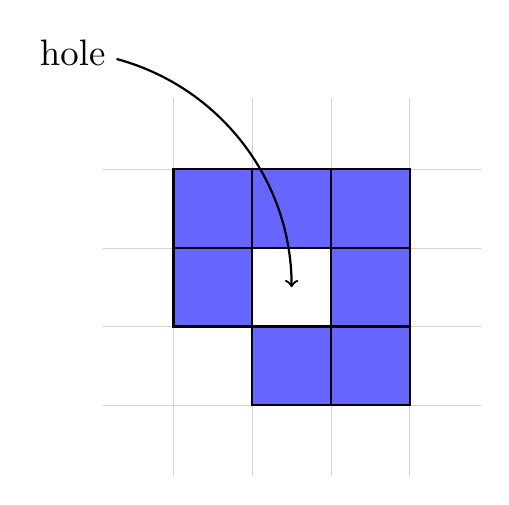
\begin{tikzpicture}
\draw[step=1cm,gray!35,very thin] (0.1,3.1) grid (4.9,7.9);

\filldraw[blue!60, draw=black, thick] (1,5) rectangle (2,6);
\filldraw[blue!60, draw=black, thick] (2,4) rectangle (3,5);
\filldraw[blue!60, draw=black, thick] (3,4) rectangle (4,5);
\filldraw[blue!60, draw=black, thick] (1,6) rectangle (2,7);
\filldraw[blue!60, draw=black, thick] (2,6) rectangle (3,7);
\filldraw[blue!60, draw=black, thick] (3,6) rectangle (4,7);
\filldraw[blue!60, draw=black, thick] (3,5) rectangle (4,6);

\draw[thick, <-] (2.5,5.5) arc (0:75:3cm);
\draw (0.3,8.15) -- (0.3,8.15) node[anchor=south east, scale=1.33] {hole};

\end{tikzpicture}

\end{document}